\documentclass[border=4pt,tikz]{standalone}
\usepackage{tikz}
\usetikzlibrary{positioning,arrows.meta,shapes.geometric,calc}
\begin{document}
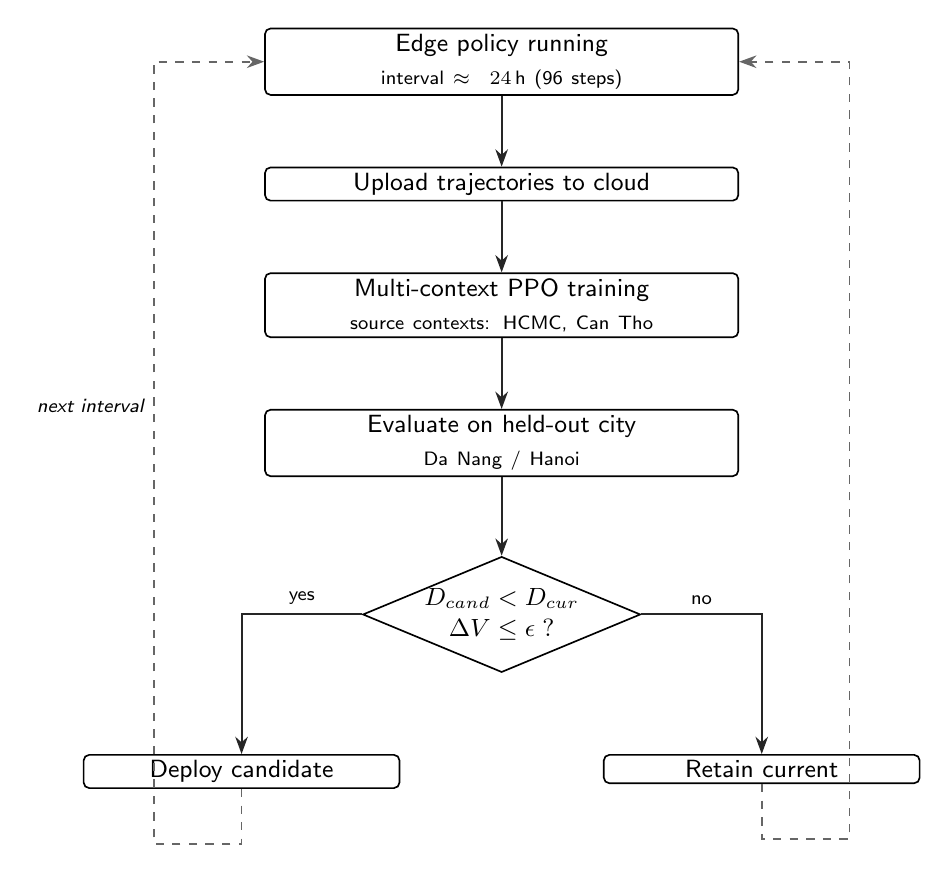
\begin{tikzpicture}[
    font=\sffamily\small,
    >={Stealth[length=2.2mm,width=1.6mm]},
    node distance=9mm and 14mm,
    task/.style    ={draw,rounded corners=2pt,
                     text width=58mm,align=center,
                     inner ysep=2pt,inner xsep=3pt,
                     line width=0.6pt,fill=white},
    leaf/.style    ={task,text width=38mm},
    decision/.style={draw,diamond,aspect=2.4,align=center,inner sep=0pt,
                     line width=0.6pt,fill=white},
    flow/.style    ={->,line width=0.7pt,draw=black!85},
    ret/.style     ={->,line width=0.6pt,draw=black!60,dashed}]

  \node[task] (run) {Edge policy running\\[1pt]{\scriptsize interval $\approx 24$\,h (96 steps)}};
  \node[task,below=of run] (up) {Upload trajectories to cloud};
  \node[task,below=of up]  (tr) {Multi-context PPO training\\[1pt]{\scriptsize source contexts: HCMC, Can Tho}};
  \node[task,below=of tr]  (ev) {Evaluate on held-out city\\[1pt]{\scriptsize Da Nang / Hanoi}};
  \node[decision,below=10mm of ev] (d) {$D_{\text{cand}} < D_{\text{cur}}$\\$\Delta V \le \epsilon\;?$};

  \node[leaf,below left=14mm and 4mm of d]  (yes) {Deploy candidate};
  \node[leaf,below right=14mm and 4mm of d] (no)  {Retain current};

  \draw[flow] (run)--(up);
  \draw[flow] (up)--(tr);
  \draw[flow] (tr)--(ev);
  \draw[flow] (ev)--(d);

  \draw[flow] (d.west) -| node[pos=0.25,above,font=\sffamily\scriptsize]{yes} (yes.north);
  \draw[flow] (d.east) -| node[pos=0.25,above,font=\sffamily\scriptsize]{no}  (no.north);

  % Return arrows curve outside, no crossings
  \draw[ret] (yes.south) -- ++(0,-7mm) -|
        ($(run.west)+(-14mm,0)$)
        node[pos=0.78,left,font=\sffamily\scriptsize\itshape]{next interval}
        |- (run.west);
  \draw[ret] (no.south) -- ++(0,-7mm) -|
        ($(run.east)+(14mm,0)$) |- (run.east);
\end{tikzpicture}
\end{document}
